\subsection{Main Unit}
\subsubsection{Block Diagram}
\createfigurewsvg{../Modular Design/Main-Unit/Figures/bdv5-main.svg}{Main Unit Architectural Diagram}{fig:bd-module-main-unit}
\subsubsection{State Diagram}
\begin{landscape}
\begin{figure}[!ht]
\begin{center}
  \begin{subfigure}[b]{0.6\textwidth}
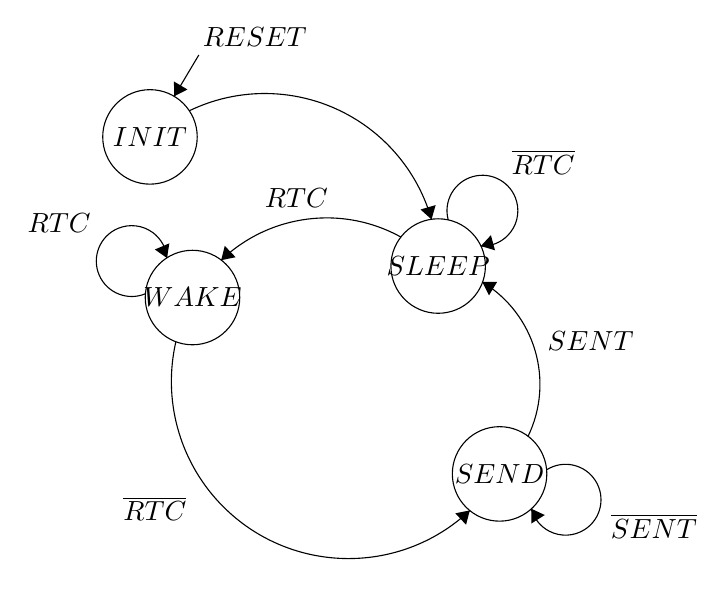
\begin{tikzpicture}[scale=0.2]
\tikzstyle{every node}+=[inner sep=0pt]
\draw [black] (36.8,-8) circle (3);
\draw (36.8,-8) node {$INIT$};
\draw [black] (55.1,-16.2) circle (3);
\draw (55.1,-16.2) node {$SLEEP$};
\draw [black] (39.5,-18.2) circle (3);
\draw (39.5,-18.2) node {$WAKE$};
\draw [black] (59,-29.4) circle (3);
\draw (59,-29.4) node {$SEND$};
\draw [black] (39.9,-2.8) -- (38.34,-5.42);
\draw (43.45,-2.3) node [above] {$RESET$};
\fill [black] (38.34,-5.42) -- (39.18,-4.99) -- (38.32,-4.48);
\draw [black] (39.29,-6.344) arc (115.82686:15.90003:11.012);
\fill [black] (54.68,-13.24) -- (54.94,-12.33) -- (53.98,-12.61);
\draw [black] (55.741,-13.281) arc (195.34019:-92.65981:2.25);
\draw (61.76,-10.43) node [above] {$\overline{RTC}$};
\fill [black] (57.81,-14.93) -- (58.71,-15.2) -- (58.45,-14.24);
\draw [black] (41.319,-15.829) arc (133.66152:60.95:9.714);
\fill [black] (41.32,-15.83) -- (42.24,-15.64) -- (41.55,-14.92);
\draw (46.1,-12.5) node [above] {$RTC$};
\draw [black] (57.903,-17.214) arc (58.79222:-25.87219:7.596);
\fill [black] (57.9,-17.21) -- (58.33,-18.06) -- (58.85,-17.2);
\draw (62.02,-20.97) node [right] {$SENT$};
\draw [black] (57.113,-31.721) arc (-46.74993:-192.99266:11.248);
\fill [black] (57.11,-31.72) -- (56.19,-31.9) -- (56.87,-32.63);
\draw (37.11,-30.8) node [below] {$\overline{RTC}$};
\draw [black] (61.977,-29.145) arc (122.62938:-165.37062:2.25);
\draw (66.04,-32.72) node [right] {$\overline{SENT}$};
\fill [black] (61.01,-31.61) -- (61.02,-32.55) -- (61.87,-32.01);
\draw [black] (36.522,-17.955) arc (293.03624:5.03624:2.25);
\draw (33.07,-13.46) node [left] {$RTC$};
\fill [black] (37.88,-15.69) -- (38.03,-14.76) -- (37.11,-15.15);
\end{tikzpicture}
\caption{Main Unit Functional State Diagram}
\label{fig:main-unit-modular-fsd-img}
  \end{subfigure}
  \begin{subfigure}[b]{0.5\textwidth}
      \begin{tabular}{c|ccc}
        STATE&\multicolumn{3}{c}{OUTPUTS}\\
        \hline
        &&&\\
        INIT&$RESET$&$\overline{RTC}$&$\overline{SENT}$\\
        SLEEP&$\overline{RESET}$&$\overline{RTC}$&$\overline{SENT}$\\
        WAKE&$\overline{RESET}$&$RTC$&$\overline{SENT}$\\
        SEND&$\overline{RESET}$&$\overline{RTC}$&$\overline{SENT}$\\
      \end{tabular}
      \caption{Main Unit Functional State Diagram: State and Outputs}
      \label{fig:main-unit-modular-fsd-state-outputs}
  \end{subfigure}
  \begin{subfigure}[b]{0.5\textwidth}
   \begin{tabular}{|c|}
    \hline
     Output List\\
    \hline
     RESET = Power on Reset\\
     SLEEP = MCU is in LPM3\\
     WAKE = RTC Timer turned on MCU\\
     SEND = Bluetooth module is sending data\\
    \hline
   \end{tabular}
      \caption{Main Unit Functional State Diagram: Output List}
      \label{fig:main-unit-modular-fsd-outputs-list}
  \end{subfigure}
\end{center}
\caption{Main Unit Functional State Diagram}
\label{fig:main-unit-modular-fsd}
\end{figure}
\end{landscape}

\subsubsection{Schematic Diagram}
\begin{landscape}
  \begin{center}
  \begin{figure}[H]
    
\includegraphics[width=\pdfpagewidth,height=0.65\textheight]{../Modular Design/Main-Unit/Figures/main-unit-and-psu.png}
    \caption{Main Unit with PSU Schematic}
    \label{fig:main-with-psu-schematic}
  \end{figure}
  \end{center}
  \end{landscape}
\subsubsection{Power Analysis}
\subsubsection{Loading, Driving, and Compatibility}
The Main Unit consists of the MSP430FR2110IPW16 MCU and the HM-10 Bluetooth module. For the MCU, it has an input voltage range from 1.8\si{\V} to 3.6\si{\V} according to it's data sheet \cite{MSP430FR2110IPW16R}. Meanwhile, the HM-10 Bluetooth module has an input voltage from 3.6\si{\V} to 6\si{\V} according to it's product listing \cite{AmazonComHiLetgo}. Due to this the MSP430FR2110 has to be supplied by the 3.3\si{V} output of the PSU and the HM-10 has to be supplied by the 5\si{\V} output of the power supply.\\
For the power available pin, according to the MSP430FR2110 data sheet, the GPIO pins can handle up to VDD =0.3\si{\V}, since in this design VDD is 3.3\si{\V} and the power available pin is at 3.3\si{\V}, it is compatible with the power sense input.\\
In order to calculate the resistor values for the green and red LEDs we used the following formula:
\begin{equation}
R = \frac{V_{cc} - V_{f}}{I_{f}}
\end{equation}
Where VCC is 3.3\si{\V} $V_{f}$ is the forward voltage for each LED and $I_{f}$ is the forward current for each LED. For the green LED \cite{GreenDiffused5mmStandard} it has a forward voltage of 2.25\si{\V} and since the MCU has a max I/O current of 2\si{\mA}, this would mean that it requires a 525\si{\ohm} resistor. Similarly, for the RED LED, it has a 2\si{\V} forward voltage and a max I/O current of 2\si{\mA}, this gives us a resistor value of  650\si{\ohm}.\\\\
Finally, for the temperature sensor (U5) \cite{TMP36GT9Z} and operational amplifier (U4) \cite{MCP6022I}, they both can be supplied by a 3.3\si{\V} supply and thus are compatible. Since the temperature sensor range for this application will be from 0\si{\celsius} to 40\si{\celsius}, at a resolution of 0.1\si{\celsius}, since there is an offset of 0.5\si{\V} by the temperature sensor gives us a range of 900 unique values so that the temperature sensor can reach its full negative temperature range. At 40\si{\celsius} the temperature sensor will be at 900\si{\milli\volt}, setting the ADC to use a 1.5\si{\V} reference. gives us a $A_{v}$ of 1.666. Setting up the op amp in a non inverting configuration, using 1\si{\kilo\ohm}, 620\si{\ohm}, 39\si{\ohm} and 5.1\si{\ohm} resistors will yield a $A_{v}$ of 1.6642.
\subsubsection{Base Times and Timing Analysis}
In order to connect both devices to each other, for communication, the best protocol to use will be UART. The MSP430FR2110 has 4 pins for UART communication using the eUSCI modules, which can detect automatically the baud-rate to be used. According to the datasheet for the HM-10 module\cite{AmazonComHiLetgo}, it can select the baud-rate to be used, which ranges from a minimum 1200 to a maximum of 230400. In the datasheet of the MSP430FR2110, the eUSCI clock frequency, UART mode, can reach a maximum of 5MHz, which means it can reach the maximum baud-rate of the Bluetooth module and can also select lower baud-rates, according to the formula:
\begin{equation}
	Clk Frequency = Baudrate \cdot 16
	\label{eq:UART Frequency}
\end{equation}
This means if we select the maximum baud-rate of the HM-10 module, which is 230400, using the formula, we would need a frequency of 3.68MHz, which is still below the maximum frequency the eUSCI module on the MSP430FR2110. This will allow us to be able to use the HM-10 communicate via UART with the MSP430FR2110.\\
\subsubsection{Software Support}
\createfigurel{../Modular Design/Main-Unit/Figures/main-unit-main-function.png}{Main Unit Main Function}{fig:main-unit-main-function}
The main function is used to:
  \begin{itemize}
    \item Initialize the RTC and to set the current time.
    \item Initialize the uart to 9600 baud for the bluetooth module.
    \item Enable global interrupts.
    \item Activate low power mode.
  \end{itemize}
\createfigurew{../Modular Design/Main-Unit/Figures/main-unit-rtc-isr.png}{Main Unit RTC ISR}{fig:main-unit-rtc-isr}
This is the error verification subroutine that runs periodically, it checks if mains power is available and assigns a boolean variable depending on the availability of mains power and then captures the current time from the RTC. Then writes the current time, power status, error from the sub unit (if any are raised) to the bluetooth TX buffer
\createfigurew{../Modular Design/Main-Unit/Figures/main-unit-bluetooth-isr.png}{Main Unit Bluetooth ISR}{fig:main-unit-bluetooth-isr}
If the interrupt is from the receiver, it will write the incoming message to the BTRXBUF until the UART goes idle. If the interrupt is from the transmitter, it first checks weather the buffer has contents, if it does, it transmits the message until a null terminator character.
\subsubsection{Memory Requirements}
The program itself consists of 300 instructions, which assuming a 1 to 10 conversion ration between C and Assembly language yields a total of 3000 bytes of program data. Since the main unit's source code has two buffers for RX and TX of 83 bytes each plus the buffer for lot number (30 bytes), the string versions of the error enums (56 bytes), the error enum (1 byte) and the error state (1 byte) gives us a size of 344 bytes of data memory.
\subsubsection{Reliability \& Design Criteria}
The main unit was the backbone of the whole system, without it there cannot be communication from the sub units to the main unit. Therefore, reliability for the main unit has to be at 100\%. Using a battle tested platform such as the MSP430FR2310 was a paramount choice in assuring the reliability of the system that ensures the safety of life saving medication. Power efficiency for the main unit is not such of a great concern since it will ideally will operate on mains power always but since the power supply has a battery backup system it can virtually guarantee 100\% reliability.
\subsubsection{Level of Completion}
\begin{landscape}
  \begin{table}[!ht]
    \begin{tabularx}{\textwidth}{|X|X|}
      \hline
      \multicolumn{2}{|X|}{Main Unit}\\
      \hline
      Integration&\begin{itemize}
                    \item Battery Backup Mains Power Supply
                    \item Main Unit
                  \end{itemize}\\
                  \hline
      Functionality&\begin{itemize}
          \item ADC 12 Initialization using VEREF+ and VEREF- reference and input channel 7.
          \item UART initialization at 9600 baud with receiver interrupts enabled.
          \item Forwards errors from sub units along with the current time.
          \item Verifies the availability of mains power and forwards that information to the host computer.
        \end{itemize}\\
      \hline
    \end{tabularx}
    \caption{Main Unit Level of Completion Table}
    \label{tab:main-unit-modular-completion-table}
  \end{table}
\end{landscape}
